\chapter{Request-based Distributed Applications}
\label{sec:requ-based-distr}

A distributed application consists of a number of processes running on
one or more servers that are communicating over a network, for the
purposes of this work, the Internet. Such applications are especially
prone to software bugs~\cite{Ballou2008}. Software bugs are defects in
a program that developers introduce through an error in thinking. If
the defective code is executed it causes an infection of the execution
state. If this infection propagates to other states, it may eventually
become visible in form of a failure~\cite{zeller2009programs}. In this
work we focus on debugging distributed Web applications, but our
approach is applicable to other distributed applications as well.

Web applications are applications accessible through a Web browser,
with, at least, a client-side component for interaction and a
server-side component for data storage. Clients are written in
JavaScript to run in the browser, and the server components may use
any programming language. Many Web applications use \ac{http} as
transfer protocol, with event-loops to handle asynchronous
communication. The reason for this is the single-threaded nature of
JavaScript in modern browsers. In the absence of multiple threads or
processes, event loops are the only option to process multiple network
events in parallel on the client. However, developers increasingly
employ event loops for server implementations as well. Event loops
avoid spawning large numbers of threads or processes that are---due to
the potentially high network latencies across wide-area
network---waiting for IO most of the time. Web applications have at
least a client and a server component, but both often communicate with
other services. These, \emph{asynchronous request-based, distributed,
multi-language applications}, are the subset of applications this work
is aimed at.

The communication patterns of many distributed systems on the Web can
be described using \ac{uml} sequence
diagrams~\cite{rumbaugh2004unified}. In a sequence diagram, each
server is an entity with a lifeline for request handling, and receives
and sends asynchronous requests. Even though \ac{http} is a
synchronous protocol, if we regard both requests and responses as
asynchronous requests, we can treat servers that handle parallel
request using any mechanism as a single thread with only asynchronous
request-handling using event-loops.

\section{Motivating Example}
\label{sec:motivating-example}

We now present an example system that uses asynchronous communication
between multiple servers. Meta-crawlers are a type of Web search
engine that connect to other search engines. Meta-crawlers combine
information from other sources and provide a unified interface to
interact with that information. For example, flight booking systems
that offer multiple airlines connect to the systems of the different
airlines and provide a unified search and booking interface to
customers. Meta-crawlers such as these offer more than just search
across multiple providers, they provide additional services for
comparing prices, comparing seating options, or booking flights.

\subsection{System Description}
\label{sec:system-description}

We have built a system that implements such a meta-crawler and is
connected to a service providing fake airline data. It consists of a
Web site that allows the user to search for and reserve flights from
an origin to a destination on a specific date. The server serving the
Web site communicates with a cache. That cache provides flight
information and caches it for a certain amount of time. Such flight
information includes flight numbers, origin and destination of
flights, information about intermediate airports for a flight, as well
as pricing and available seats. This cache, in turn, connects to a
flight-data generator service that stands in for the airlines
providing information about their scheduled flights. All communication
is done via \ac{json}\footnote{JavaScript Object Notation\\
\url{http://www.ietf.org/rfc/rfc4627.txt}\\ accessed July 25,
2012}. The setup for this system is shown if
\autoref{fig:flyhehe-setup}, with the arrows indicating data
direction.

An intermediate query and cache service is an optimization that
meta-crawlers use, which avoids having to query the data sources
directly on each user request. Querying on each request is undesirable
due to network latencies and because data providers usually limit the
number of queries per time unit that meta-services can send to save
bandwidth and processing time. However, caches introduce the problems
of stale data and cache invalidation. Prices for seats on airplanes
usually rise as the flight date approaches, and as increasingly fewer
seats are available. Consequently, in order to create a reservation,
flight booking systems either cannot guarantee the exact prices for
their results, or they have to invalidate their caches and query for
current data at the time of reservation.

\begin{figure}
  \centering
  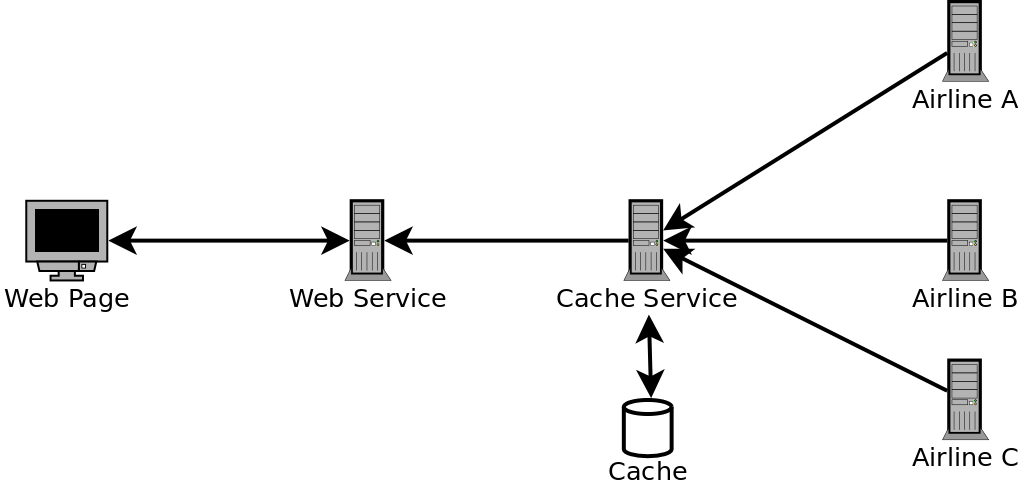
\includegraphics[width=0.7\linewidth]{flyhehe-setup}
  \caption{Flight Meta-Crawler Demo Setup}
  \label{fig:flyhehe-setup}
\end{figure}

\subsection{Failure Scenarios}
\label{sec:failure-scenarios}

Consider two customers on the meta-crawler Web page at the same
time. Both are looking for flights from Berlin to Amsterdam, as shown
in \autoref{fig:flyhehe}. The results of their search will be served
from the cache, and may not be the most recent data from the
respective airlines. If both customers try to reserve seats on flight
\emph{LH1009} at roughly the same time, different things may happen.

First, depending on the geographical location of both users with
respect to our system, the request for reservation may take some time
to reach the server. Depending on the time difference, one reservation
may complete entirely before the other request even arrives at the
server. As we have said above, in order to create a guaranteed
reservation, the Web server has to query the airline data---or, in our
case, the fake airline data generator---for the most recent rates and
available seats. Let us assume that the cache data was current and the
first reservation request can be fulfilled at the displayed rate of
156 EUR. By the time the second request for reservation arrives at the
Web server, the number of available seats has thus gone down to one,
which means the prices has gone up as the airline adjusts pricing
depending on available seats. Thus the second reservation can also
complete, but only at a higher rate.

Second, it may be that both requests for reservation \emph{arrive} at
our server at the same time, and are served in parallel. This leads to
a race condition for which we cannot deterministically decide which
one of the users receives the lower rate and which one the higher
rate. Either way, we, as the provider of the meta-service, do not want
to end up reserving two seats and receiving only the lower rate from
both customers, because in that case, depending on our and the
airlines' terms of service, we may have to pay the price difference or
a fine, which may not be a sustainable way to make business. At the
same time, as a customer, we do not want to create a binding
reservation at any other rate than the one shown on the Web site at
the time of our click on the \emph{Reserve Seat} link.

\begin{figure}
  \centering
  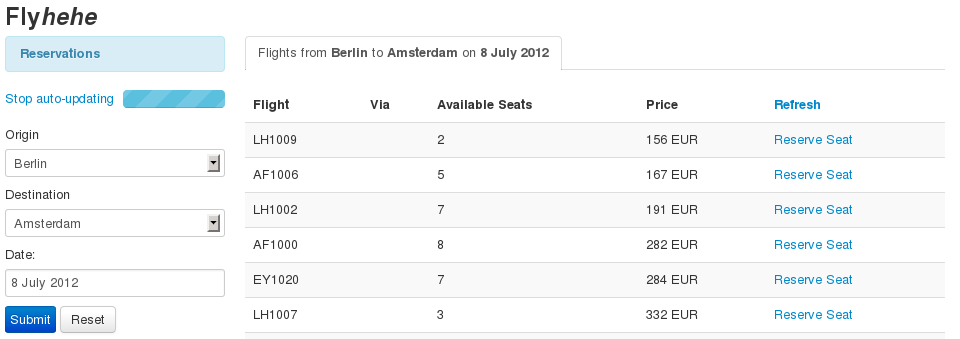
\includegraphics[width=\linewidth]{flyhehe}
  \caption{Flight Meta-Crawler Demo System}
  \label{fig:flyhehe}
\end{figure}

There are a number of challenges for the developers of such a
system. First, they have to understand the communication patterns that
may arise in production, with parallel access to the Web site, cache,
and airline data. They have to implement ways to deal with data races
and non-determinism caused by network delays. To do that, they have to
understand how non-determinism may lead to undesired states in their
application, such as making a wrong reservation. To verify their
solutions, they need a way to reliably reproduce problems and test
them. Finally, they need to understand how communication between two
systems tightly couples them at the implementation level, which means
they have to understand how changes to the code in one system may
impact that systems' ability to communicate with the others.

\subsection{From Bug Report to Failure}
\label{sec:from-bug-report}

A bug is an expression of a defect as a visible failure in the output
of a system. To fix a bug, developers have to understand the failure,
find the underlying defect, and remove it. Imagine the following bug
report for our flight booking system:

\begin{quote}
  Sometimes, when I try to book a flight on your website,
  it is added to my cart just fine, but with a different price than what
  it was in the list when I clicked it.
\end{quote}

This particular bug report is at a high abstraction level, as it
describes only user-facing input and effects. For such bug reports,
the first step towards fixing them is to reproduce them. Second,
developers should write a minimal piece of executable code that
reproduces the failure, so they can easily check their attempts at a
fix. Then the actual process of debugging can begin, which will
eventually make the test case pass.

These steps can be time-consuming, especially for very abstract bug
reports. Tools such as \emph{ReCrash}~\cite{Artzi} attempt to generate
test cases automatically, but can only do so for deterministic
failures. The above bug report contains the word "sometimes",
indicating a degree of non-determinism. That non-determinism may have
a number of causes. In this case, it may be that the user attempts to
book flights slightly differently without noticing. There may be
conditions in the environment, from browser bugs to transient hardware
failures, that cause the issue to only appear sporadically. Or there
may be non-determinism in the Web server implementation or the network
communication.

To approach non-determinism during debugging, developers have to check
each possible cause and try to eliminate it. Most of these causes,
including network communication, are difficult to reproduce faithfully
outside the live system. Unit tests are likely to be too low-level to
expose complex interactions, and acceptance tests running in a test
setup experience different conditions if the test setup is not
similar enough to the live system. Developers cannot with certainty
know whether a test setup sufficiently models the live system to
reproduce a given failure.

Given the above bug report and its possible causes, developers at some
point have to inspect the network communication schedule if no other
cause can be found.

\paragraph{Scripted Diagnoses}
\label{sec:scripted-clients}

Instead of acceptance or unit tests in controlled test environments,
developers may employ \emph{system diagnoses} as "test cases" to
simulate user input against the live system. Oftentimes those are
simple scripts simulating a browser's communication with the Web
page. This enables developers to include the circumstances under which
the bug occurred in the test. Even if the bug only occurs "sometimes",
repeated execution of the system diagnosis will eventually reproduce
it if it is related to varying network schedules.

This is the approach taken by tools such as
\emph{iDNA}~\cite{Bhansali2006} and statistical debugging
approaches. The deployed application is observed over long periods of
time, possibly through multiple occurrences of the failure. If the
failure occurs, as established by the bug report, "sometimes", then
the diagnosis is good enough for Replay-driven Fault Navigation.

\section{Challenges when Debugging in Distributed Environments}
\label{sec:debugg-distr-envir}

In distributed systems such as our flight booking system, developers
face a set of challenges in addition to the challenges of
non-distributed systems. The implementation of each service has to
account for the unreliable network, developers need to understand the
services they communicate with, and how data is represented and shared
between those
services.\\

\begin{description}
\item[Non-determinism] Non-determinism may have different causes: from
  randomness in the implementation, varying shared resource access
  order, to interactions with other processes and the operating system
  schedule and transient faults in hardware. Non-determinism here
  means that for equal inputs, the output and execution speed of a
  program is indeterminate.

  For a distributed system, non-determinism may mean that for an equal
  number and order of messages sent from one server, another server
  may produce different responses. A cause unique to distributed
  systems for this is network latency and request re-ordering. Sending
  a number of \ac{http} requests in one particular order does not
  guarantee its delivery in the same order. This is an instance of a
  leaky abstraction. \ac{http} messages may be broken up into multiple
  \ac{tcp} packets. \ac{tcp} packets may arrive out of order, and are
  collected by the operating system and delivered to applications in
  the original order for a connection. If the \ac{tcp} packets for one
  \ac{http} connection are available, the operating system passes
  those packets to the application, which handles them as \ac{http}
  request. The application does not know that another \ac{http}
  request is on its way that was sent earlier from the point of view
  of the sender. So, if the processing of any request is influenced by
  any other, network latency may introduce non-determinism.

  Network latency varies across network segments. Usually, during
  development, distributed systems are deployed in a test environment
  in an attempt to simulate the distribution properties of the
  deployed system. However, actual network latency during deployment
  is hard to predict, and data races across the network will only
  randomly be reproduced in a test environment. Furthermore, during
  development, \emph{click-races}---the situation when two or more
  users try access a resource simultaneously---can oftentimes not be
  adequately tested. Finally, deployed distributed systems, due to
  ongoing communication, very rarely enter a globally consistent
  state, so proving a system correct for its projected uptime is
  difficult~\cite{Geels2006Replay}. The only predictable way to enter
  consistent states is to shut down and restart the whole system
  regularly, which is not desirable for many systems.
\item[Heisenbugs] Failures that occur only during or change during
  debugging are called \emph{Heisenbugs}~\cite{Gray1986}. They happen
  because the debugging tool, through its observation process, changes
  the runtime behavior of the observed program. For non-deterministic
  failures, this means that introducing logging into the system may
  cause different failures to happen, or the original failure could
  happen much more or much less frequently, or not at all. This makes
  debugging non-deterministic failures harder, because the developer
  cannot be sure that the observed failure is the same as the original
  one.

  Distributed systems exhibit Heisenbugs more often, because network
  access order varies even from slight disturbances, such as the
  operating system scheduler or other processes in the system. Most
  debuggers incur significant overhead~\cite{Corliss2005}, which
  causes equally great disturbances to network access order, which in
  turn may cause Heisenbugs~\cite{Gait1985}.
\item[Languages] When systems run on different machines, or even only
  in different processes, and they communicate not via the language
  calling mechanisms, but rather through foreign-function interfaces,
  shared memory, or network communication, connecting call trees in
  one language to another is a non-trivial task.

  A developer has to find exit and entry points for \ac{ipc} in all
  communicating systems, and relate the input and output data, to
  connect events within one system to another. This task is made more
  difficult by abstractions from the input and output, for example,
  while the operating system will deliver \ac{tcp} packets in order to
  a language runtime, a Web framework will assemble \ac{http} messages
  before passing the data on to the application. If systems use
  different abstractions, one working on the transport layer and the
  other on the application layer, it is hard to determine the
  corresponding communication entry points.
\item[Data Representation] Different languages represent data
  differently. Consequently, different kinds of persistent data
  representation come natural to the language users. Different data
  representations have to be converted into each other, which
  introduces additional complexity and another source for
  bugs. Because the connection between the different systems and the
  data conversion is usually hidden behind libraries and frameworks,
  failures that are caused by incorrect data exchange are hard to
  debug, because developers have to understand multiple systems and
  how they transform the data.

  For example, a web-page will naturally display information to a user
  in a visual manner, using nested \textsc{HTML}-\textsc{DOM} elements
  to express the information content in a user-friendly way. The
  JavaScript code running in the browser will usually, at least
  intermittently, store information as JavaScript objects or in
  \ac{json}. \ac{json} may also be the format used in \ac{http}
  requests to transfer data between the client and the server. On the
  server, the data may again be transformed any number of times
  between different runtimes, backend servers, and databases.
\end{description}
~\\
These properties make debugging distributed systems a laborious
task. We have identified the following four debugging activities to be
especially problematic and in need of a solution.

\subsection{Observation and Logging}
\label{sec:observation-logging}

The need for observation and logging of program state changes has
clearly been recognized in both research and
industry~\cite{Saito2005,altekar2009odr,Stanley2009}. Most Web
frameworks include logging facilities, different log-levels, and
separate logs for access, input, output, erroneous and successful
events. There are full libraries\footnote{Airbrake: The error app 
  \url{https://airbrake.io/pages/home}\\
  accessed June 25, 2012} and frameworks\footnote{Apache log4j
  Logging Services
  \url{http://logging.apache.org/log4j/1.2/index.html}\\
  accessed June 25, 2012}
that provide comprehensive logging facilities to applications.

Distributed system are setup differently during development than at
deployment time. Simulation of distributed systems or parts thereof in
small-scale development deployments, as used at development time of
such systems, allows developers to evaluate system behavior in a
simple setting, relative to the deployment setup. In such development
setups, developers have full control over each server, and the power
to stop and inspect each process at practically any point in the
execution of the distributed system. Apart from such small-scale
setups, developers use full-scale test deployments to provide a more
realistic setting for stress testing critical aspects of the
system. Using setups of varying degree between fully local deployments
and full-scale test environments, developers can control the amount of
realism their code is exposed to.

However, once deployed, distributed systems will over time encounter
situations that could not have been anticipated by the developers,
state changes accumulate, the underlying network topology changes,
and, for successful services, system load and parallelism increases
beyond what could reasonably be
tested~\cite{Geels2006Replay}. Long-running applications may
experience non-deterministic, low-probability failures that develop
over time. Thus, logging data from the deployed system is
indispensable for testing and debugging failures that occur during
deployment.

If problems occur, most logging frameworks have settings on how to
react, by sending emails, checkpointing the running application,
stopping and saving a stack-dump of the program state,
etc. \emph{heartbeat} services regularly check accessibility of
services, existence of error artifacts, or output of logging
frameworks, to filter and notify developers when a problem occurs in
the deployed system.

Logging frameworks and error artifacts are useful for debugging, as
long as only a limited number of frameworks is used. As long as logs
are similar in format and level of abstraction, they can be related to
one another. However, although most frameworks that are used in the
context of networked applications offer logging capabilities, there is
no widely accepted standard for logging information and formats across
languages or frameworks.

\subsection{Understanding and Classifying Observations}
\label{sec:distr-reas}

Given appropriate logging, developers have to review and understand
the logs to determine how to approach a particular bug. This entails
associating parts of a log or particular log entries with
failures. Even for stack traces of single process applications, this
is no easy task, and developers can easily get confused about where to
look first in a trace~\cite{groetker2012Tdg}. For Web applications
developers have to understand and associate parts of logs from
different systems with the same failures. As different logs may expose
different aspects of the same problem, they have to be aligned with
respect to their order, so developers have chain of anomalous log
entries to follow backwards. Without such alignment, developers can
only guess which anomaly occurred first, and finding the cause of a
failure is a matter of trial and error. But aligning multiple logs is
a difficult task, unless there is a connected logging
facility. Minimal clock skew across systems may render timestamps
unusable for log ordering and parallel events cannot easily be
recognized as such.

Another problem presents itself when the failure is logged at a
different level of abstraction than the anomalies leading up to it.
For example, if the log entry with \ac{http} status code 500 on the
server represents the visible failure, the anomalies leading up to it
may be in form of database access or JavaScript exceptions, but there
may be multiple database accesses or exceptions for only one \ac{http}
request. Developers have to connect these anomalies and group them at
the right level of abstractions. Thus, understanding which log entries
are relevant to a particular failure is hard to determine as well.

\subsection{Reproducing Failures}
\label{sec:reproducing-failures}

Many debugging guides emphasize that the ability to reliably reproduce
a failure is crucial in the attempt to fix the underlying defect,
because it is the only way to make sure that an attempted fix is
successful~\cite{metzger2003Dbt,zeller2009programs,groetker2012Tdg}. This
can be difficult for single-process applications, however, distributed
applications exacerbate this problem. The \emph{global state} in a
distributed system is hardly ever consistent, unless the whole system
is restarted. That means that there is little opportunity for
checkpointing the system for running through a failure from the
checkpoint. To checkpoint a process, it needs to be in a consistent
state, so it can restarted later. For multiple processes, this means
that all nodes---and thus the complete distributed system---have to be
in a well-known state before a checkpoint.

Provided a consistent checkpoint can be established \emph{before} a
failure occurs, reproduction may still fail. Non-deterministic
failures caused by network latency or transient inconsistency in the
global state will not manifest each time the defective code is
triggered.

To deal with this problem, there are approaches to log \ac{http}
traffic on-demand, when a failure occurs~\cite{Konuru2000}. During
replay, instead of just running the complete, distributed system, only
one node is actually run, and interaction with external services is
replayed from records.

This is useful if the developer knows on which node the defect is most
likely to find. If that is unclear, however, the developer can only
replay and debug on each node, sequentially, until the defect is
found. For large numbers of communicating nodes, or if the error is
not on any node the developer can access, this is a time-consuming
process that may not lead to success.

\subsection{Connecting Server Events to Code Locations}
\label{sec:conn-serv-code}

Provided a useful log and a replay mechanism exist, and developers
have identified server events and servers that contribute to a
failure, they have to change the level abstraction from network
communication and servers to communicating processes and source code
to find and fix the defect. In distributed systems, it is not possible
to set a \emph{breakpoint} on a network event, and stop all services
that are communicating at the time to inspect them.

In order to deal with this problem, developers use logging in
different ways. Simple logging mechanisms or frameworks can be used to
determine the executed code around a particular network event. This
increased logging can be enabled on-demand, and log, for example,
method activations, arguments, and the data that is sent and received
over the network~\cite{Artzi}. Another approach is to save a full
continuation of the running program when a particular event
occurs~\cite{ducasse2010dynamic}. This continuation can later be
inspected with a symbolic debugger.

The problem with these approaches is that they only provide a
one-to-one connection between a network event and a code
location. Yet, code locations are connected across servers via the
network, so multiple code locations contribute to the same
request. Developers need to identify the same network events as they
are logged on different servers, to find those connections, and the
debugging tools have to provide this identification.

\subsubsection{Working with Multiple Call Trees}
\label{sec:work-with-mult}

Debugging across communicating processes is similar to debugging
across multiple threads. First, in both cases it is impossible to stop
all execution in one atomic step. Second, all processes and threads
have a separate stack as well. However, in contrast to multi-threaded
applications, distributed applications cannot communicate through
shared memory and have to use an \ac{ipc} mechanisms instead. In the
case of Web applications, \ac{http} \acp{api} are the \ac{ipc}
mechanism.

Consider again the sequence diagram for expressing the runtime
behavior of distributed systems. As per the \ac{uml} standard, nested
calls can be expressed using nested lifelines. Generally, that would
be the case if a method call from one object to another causes the
receiver to call another method on itself or a third object. For
distributed applications, this can describe the relation of network
messages and call trees. An \ac{http} request will trigger some code
to be executed on the receiver. While the level of abstraction is
different, in effect, this is equal to communicating threads and their
interleaved call trees.

Each node executes code in one language, on one or more threads. The
language runtime takes care of delivering calls to and return values
from call-sites. On the network, the \ac{http} layer has that
responsibility. This means, that in distributed systems there are
multiple, nested layers of \emph{runtimes}, each with their own call
mechanism.

Developers of multi-threaded programs need to be able to move between
call trees freely. The same applies for developers of distributed
systems. While thread call trees within one runtime are at the same
level of abstraction, network call trees and different language
runtimes are not. There is very little support for connecting those
layers within debugging tools, and methods for doing so are still
being researched~\cite{Stanley2009,Geels2006Replay}.

%%% Local Variables: 
%%% mode: latex
%%% TeX-master: "thesis"
%%% End: 
